\documentclass[a4paper, 12pt]{report}

\usepackage[utf8]{inputenc}
\usepackage[T1]{fontenc}
\usepackage{lmodern}
\usepackage[ngerman]{babel}
\usepackage[margin=3.0cm,top=4cm]{geometry}
\usepackage[]{graphicx}

\usepackage{array}
\usepackage{lastpage}
\usepackage{blindtext} 
\usepackage{amsmath} 
\usepackage{nicefrac}
\usepackage{float}


\newcolumntype{L}[1]{>{\raggedright\let\newline\\\arraybackslash\hspace{0pt}}m{#1}}
\newcolumntype{C}[1]{>{\centering\let\newline\\\arraybackslash\hspace{0pt}}m{#1}}
\newcolumntype{R}[1]{>{\raggedleft\let\newline\\\arraybackslash\hspace{0pt}}m{#1}}


\usepackage{sectsty}
\sectionfont{\fontsize{15}{15}\selectfont}
\subsectionfont{\fontsize{12}{15}\selectfont}

\renewcommand{\familydefault}{\sfdefault}

\usepackage{fancyhdr}

\pagestyle{fancy}
\fancyhf{}
\fancyhead[L]{Grundbegriffe}
\fancyhead[R]{Stefan Urban}
\fancyfoot[R]{Seite \thepage\ von \pageref{LastPage}}
\renewcommand{\headrulewidth}{0.4pt}

%\addtolength{\parskip}{2mm}
\setlength{\parindent}{0pt}


\begin{document}


\section*{Relationen}

	\subsection*{Definitionen}
	
	\begin{center}
		\begin{tabular}{|c|l|}
			\hline Dekade & 10 zu 1 \\ 
			\hline Oktave & 2 zu 1 \\ 
			\hline Terz & $ \sqrt[3]{2} = 1,26 $ zu 1 \\ 
			\hline 
		\end{tabular}
	\end{center}
	
	\subsection*{Umrechnungen}
	
	Zusammenhang zwischen Dekade, Oktave und Terz
	
	\begin{center}
		1 Dekade = 10 Terzen
		
		1 Oktave = 3 Terzen
	\end{center}
	
	Anzahl der Dekaden / Oktaven / Terzen in einem Frequenzbereich:
	
	\[
 		Anzahl = \log_{Relation}{f_o / f_u} = \frac{\log_{10}{f_o / f_u}}{\log_{10}{Relation}}
	\]
	
	\vspace{0.5cm}

	\begin{minipage}[t]{0.3\textwidth}
		\begin{center}
			Dekaden:
		\end{center}
		\[ \log \frac{f_o}{f_u} \]
	\end{minipage}
	\begin{minipage}[t]{0.3\textwidth}
		\begin{center}
			Oktaven:
		\end{center}
		\[ \frac{\log f_o / f_u}{\log 2} \]
	\end{minipage}
	\begin{minipage}[t]{0.3\textwidth}
		\begin{center}
			Terzen:
		\end{center}
		\[ \frac{\log f_o / f_u}{\log 1,26} \]
	\end{minipage}
	
	
	\vspace*{1cm}
	
	Zusammenhang zwischen Mitten-, Oberer und Unterer Frequenz:

	{\large
		\begin{minipage}[t]{0.5\textwidth} 
			\begin{align*} 
					f_m = \sqrt{f_o  \cdot  f_u}
			\end{align*} 
		\end{minipage}
		\begin{minipage}[t]{0.5\textwidth} 
			\begin{align*} 
				\frac{f_o}{f_u} = Relation
			\end{align*} 
		\end{minipage}
	}

	\begin{minipage}[t]{0.2\textwidth} 
		\begin{align*} 
			Terz
		\end{align*} 
	\end{minipage} 
	\begin{minipage}[t]{0.4\textwidth} 
		\begin{align*} 
			f_o = f_m  \cdot  \sqrt{1,26}
		\end{align*} 
	\end{minipage}
	\begin{minipage}[t]{0.4\textwidth} 
		\begin{align*} 
			f_o = f_u \cdot 1,26
		\end{align*} 
	\end{minipage}

	\begin{minipage}[t]{0.2\textwidth} 
		\begin{align*} 
			Oktave
		\end{align*} 
	\end{minipage} 
	\begin{minipage}[t]{0.4\textwidth} 
		\begin{align*} 
			f_o = f_m  \cdot  \sqrt{2}
		\end{align*} 
	\end{minipage}
	\begin{minipage}[t]{0.4\textwidth} 
		\begin{align*} 
			f_o = f_u \cdot  2
		\end{align*} 
	\end{minipage}

	\begin{minipage}[t]{0.2\textwidth} 
		\begin{align*} 
			Dekade
		\end{align*} 
	\end{minipage} 
	\begin{minipage}[t]{0.4\textwidth} 
		\begin{align*} 
			f_o = f_m  \cdot  \sqrt{10}
		\end{align*} 
	\end{minipage}
	\begin{minipage}[t]{0.4\textwidth} 
		\begin{align*} 
			f_o = f_u \cdot 10
		\end{align*} 
	\end{minipage}
	
	
	\clearpage
	
	
	
\section*{Rosa Rauschen (RR, 1/f-Rauschen)}
	
	Gleiche Leistung in jeder Terz
	
	\[ U_{ges,RR} = U_{Terz} \cdot \sqrt{Terzen} \]
	\[ P_{ges,RR} = P_{Terz} \cdot Terzen \]
		

\section*{Weißes Rauschen (WR)}
	
	Gleiche Leistung in jedem gleich großen Frequenzband. $ 1 dBV $ pro Terz Unterschied!
	
	\[ U_{ges,WR} = U_{Terz} \cdot \sqrt{\frac{10^{\nicefrac{1}{10} \cdot Terzen} - 1}{10^{\nicefrac{1}{10}} - 1}} \]
	\[ P_{ges,WR} = Bandbreite \cdot P_x \qquad [P_x] = \frac{W}{Hz} \]


\section*{Addition von unkorrelierten Signalen}

	Die Spannungswerte können nicht einfach zusammengezählt werden. Es ist eine geometrische Addition erforderlich:
	
	{\large \[
		U_{ges} = \sqrt{U^2_{1} + U^2_{2} + ...} \qquad
		P_{ges} = P_{1} + P_{2} + ...
	\]}

	
\section*{Thermisches Rauschen eines Widerstands}

	Thermisches Rauschen ist weißes Rauschen.

	{\large 	\[ \tilde{U}_{th,LL} = e_n  \cdot  \sqrt{\Delta f} \qquad e_n = \sqrt{4 \cdot k \cdot T \cdot R} \]}
	
	Boltzman-Konstante k im Taschenrechner Kürzel 25\footnote{nur mit CASIO fx-991DE PLUS}
	
	\[ k = 1,3807 \cdot 10^{-23} \frac{J}{K} \qquad T_0 = 273,15 K
	\qquad e_{n,ges} = \sqrt{\sum e^2_n}
	\qquad e_n = i_n \cdot R
	\]
	
	Rauschleistung:
	
	{\large \[ P = \frac{\tilde{U}^2_{th,LL}}{R} \qquad \sim \frac{1}{\Delta f} \]}

\clearpage

\section*{Systemeigenschaften}

	\begin{tabular}{|p{5cm}|p{9cm}|}
	\hline Kausales System &  Ein System heißt kausal, wenn die Ausgangsgröße $ y(t_1) $ zu einem beliebigen Zeitpunkt $ t_1 $ nur
	vom Verlauf der Eingangsgröße $ u(t) $ bis zum Zeitpunkt $ t_1 \ge t $ abhängt. Bei einem kausalen System muss erst eine Ursache eintreten, bevor sich eine Wirkung zeigt. \\
	\hline Zeitinvariantes System & Ein System wird als zeitinvariant bezeichnet, wenn die Systemgleichung $ y(t) = Gu(t) $ die Verschiebungseigenschaft
	\[ G\{u(t-t_0)\} = y(t-t_0) \]
	für beliebige Verschiebungszeiten $ t_0 \ne 0 $ und alle Zeiten $ t $ besitzt. \\ 
	\hline Lineares System & Ein System ist linear, wenn es folgende Eigenschaften besitzt:
		\begin{itemize}
		\itemsep 0 em
		\parskip 0 em
		\item Proportionalität $ G\{k \cdot u(t)\} = k \cdot G\{ u(t) \} $
		\item Superposition \newline $ G\{u_1(t) + u_2(t) \} = G\{ u_1(t) \} + G\{ u_2(t) \} $
		\end{itemize} \\ 
	\hline Minimalphasiges System & Unter allen kausalen Systemen mit gleichem Amplitudengang wird
	dasjenige als „Minimalphasensystem“ bezeichnet, das den geringsten
	Phasenverzug hat. \newline Jedes System lässt sich in ein minimalphasiges System und einen Allpass zerlegen. \\ 
	\hline Linearphasiges System & Ein linearphasiges System zeichnet sich durch eine konstante Gruppenlaufzeit aus. \[ \frac{d\varphi}{df} = const. \] \\ 
	\hline
	\end{tabular}
	
\clearpage

\section*{Allgemeines Filter 1. Ordnung}

	\vspace{0.5cm}

	\begin{large}
		\[ \underline{H}(p) = k \cdot \frac{1 + ap}{1 + bp} \]
	\end{large}
	
	\vspace{-0.5cm}
	
	\subsection*{TP1 - Tiefpass 1. Ordnung}
		\begin{minipage}[t]{0.5\textwidth}
			\[ a = 0 \qquad b = \nicefrac{1}{\omega_x} \]
		\end{minipage}
		\begin{minipage}[t]{0.5\textwidth}
			\[ \underline{H}(p) = \frac{1}{1 + \nicefrac{p}{\omega_x}} \]
		\end{minipage}
	
	\subsection*{TP1g - Tiefpass 1. Ordnung mit Gegenhalt}
		\begin{minipage}[t]{0.5\textwidth}
			\[ a = \nicefrac{1}{\omega_0} \qquad b = \nicefrac{1}{\omega_x} \qquad \omega_0 > \omega_x \]
		\end{minipage}
		\begin{minipage}[t]{0.5\textwidth}
			\[ \underline{H}(p) = \frac{1 + \nicefrac{p}{\omega_0}}{1 + \nicefrac{p}{\omega_x}} \]
		\end{minipage}
	
	\subsection*{HP1 - Hochpass 1. Ordnung}
		\begin{minipage}[t]{0.5\textwidth}
			\[ a = \nicefrac{1}{\omega_x} - \nicefrac{1}{p} \qquad b = \nicefrac{1}{\omega_x} \]
		\end{minipage}
		\begin{minipage}[t]{0.5\textwidth}
			\[ \underline{H}(p) = \frac{\nicefrac{p}{\omega_x}}{1 + \nicefrac{p}{\omega_x}} \]
		\end{minipage}
	
	\subsection*{HP1g - Hochpass 1. Ordnung mit Gegenhalt}
		\begin{minipage}[t]{0.5\textwidth}
			\[ a = \nicefrac{1}{\omega_0} \qquad b = \nicefrac{1}{\omega_x} \qquad \omega_0 < \omega_x \]
		\end{minipage}
		\begin{minipage}[t]{0.5\textwidth}
			\[ \underline{H}(p) = \frac{1 + \nicefrac{p}{\omega_0}}{1 + \nicefrac{p}{\omega_x}} \]
		\end{minipage}
	
	\subsection*{AP1 - Allpass 1. Ordnung}
		\begin{minipage}[t]{0.5\textwidth}
			\vspace{-0.3cm}
			\[ a = \nicefrac{-1}{\omega_x} \qquad b = \nicefrac{1}{\omega_x} = -a \qquad k = \nicefrac{1}{2} \]
		\end{minipage}
		\begin{minipage}[t]{0.5\textwidth}
			\[ \underline{H}(p) = \frac{1 - \nicefrac{p}{\omega_x}}{1 + \nicefrac{p}{\omega_x}} \]
		\end{minipage}
		
\clearpage

\section*{Allgemeines Filter 2. Ordnung}

	\vspace{0.5cm}

	\begin{large}
		\[ \underline{H}(p) = k \cdot \frac{1 + ap + bp^2}{1 + cp + dp^2} \]
	\end{large}
	
	\vspace{-0.5cm}
	
	\subsection*{TP2 - Tiefpass 2. Ordnung}
		\begin{minipage}[t]{0.5\textwidth}
			\[ a = 0 \qquad b = 0 \]
			\[ c = \frac{1}{Q\omega_x} \qquad d = \frac{1}{\omega^2_x} \]
		\end{minipage}
		\begin{minipage}[t]{0.5\textwidth}
			\vspace{0.4cm}
			\[ \underline{H}(p) = \frac{1}{1 + \frac{p}{Q\omega_x} + \left(\frac{p}{\omega_x}\right)^2} \]
		\end{minipage}
	
	\subsection*{TP2g - Tiefpass 2. Ordnung mit Gegenhalt}
		\begin{minipage}[t]{0.5\textwidth}
			\[ a = \frac{1}{Q\omega_0} \qquad b = \frac{1}{\omega^2_0} \]
			\[ c = \frac{1}{Q\omega_x} \qquad d = \frac{1}{\omega^2_x} \]
		\end{minipage}
		\begin{minipage}[t]{0.5\textwidth}
			\[ \omega_0 > \omega_x \qquad \nicefrac{a}{c} = \nicefrac{b}{d} = \nicefrac{\omega_x}{\omega_0} < 1 \]
			\vspace{-0.2cm}
			\[ \underline{H}(p) = \frac{1 + \frac{p}{Q_0\omega_0} + \left(\frac{p}{\omega_0}\right)^2}{1 + \frac{p}{Q_x\omega_x} + \left(\frac{p}{\omega_x}\right)^2} \]
		\end{minipage}
	
	\subsection*{HP2 - Hochpass 2. Ordnung}
		\begin{minipage}[t]{0.5\textwidth}
			\[ a = 0 \qquad b = \frac{1}{\omega^2_x} \]
			\[ c = \frac{1}{Q\omega_x} \qquad d = \frac{1}{\omega^2_x} \]
		\end{minipage}
		\begin{minipage}[t]{0.5\textwidth}
			\[ b = d \]
			\vspace{-0.2cm}
			\[ \underline{H}(p) = \frac{\left(\frac{p}{\omega_x}\right)^2}{1 + \frac{p}{Q\omega_x} + \left(\frac{p}{\omega_x}\right)^2} \]
		\end{minipage}
	
	\subsection*{HP2g - Hochpass 2. Ordnung mit Gegenhalt}
		\begin{minipage}[t]{0.5\textwidth}
			\[ a = \frac{1}{Q\omega_0} \qquad b = \frac{1}{\omega^2_0} \]
			\[ c = \frac{1}{Q\omega_x} \qquad d = \frac{1}{\omega^2_x} \]
		\end{minipage}
		\begin{minipage}[t]{0.5\textwidth}
			\[ \omega_0 < \omega_x \qquad \nicefrac{a}{c} = \nicefrac{b}{d} = \nicefrac{\omega_x}{\omega_0} > 1 \]
			\vspace{-0.2cm}
			\[ \underline{H}(p) = \frac{1 + \frac{p}{Q_0\omega_0} + \left(\frac{p}{\omega_0}\right)^2}{1 + \frac{p}{Q_x\omega_x} + \left(\frac{p}{\omega_x}\right)^2} \]
		\end{minipage}
	
	\subsection*{BP2 - Bandpass 2. Ordnung}
		\begin{minipage}[t]{0.5\textwidth}
			\[ a = \frac{1}{Q\omega_x} \qquad b = \frac{-1}{p^2} \]
			\[ c = \frac{1}{Q\omega_x} \qquad d = \frac{1}{\omega^2_x} \]
		\end{minipage}
		\begin{minipage}[t]{0.5\textwidth}
			\[ a = c \]
			\vspace{-0.2cm}
			\[ \underline{H}(p) = \frac{\frac{p}{Q\omega_x}}{1 + \frac{p}{Q\omega_x} + \left(\frac{p}{\omega_x}\right)^2} \]
		\end{minipage}
		
\clearpage

	\subsection*{EQ2 - Equalizer 2. Ordnung}
		\begin{minipage}[t]{0.5\textwidth}
			\[ a = v \cdot \frac{1}{Q\omega_x} \qquad b = \frac{1}{\omega^2_x} \]
			\[ c = \frac{1}{Q\omega_x} \qquad d = \frac{1}{\omega^2_x} \]
		\end{minipage}
		\begin{minipage}[t]{0.5\textwidth}
			\[ a = v \cdot c \qquad b = d \]
			\vspace{-0.2cm}
			\[ \underline{H}(p) = \frac{1 + v\cdot\frac{p}{Q\omega_x} + \left(\frac{p}{\omega_x}\right)^2}{1 + \frac{p}{Q\omega_x} + \left(\frac{p}{\omega_x}\right)^2} \]
		\end{minipage}

	\subsection*{BS2 - Bandsperre 2. Ordnung}
		Sonderform des EQ2 mit v = 0
	
		\begin{minipage}[t]{0.5\textwidth}
			\[ a = 0 \qquad b = \frac{1}{\omega^2_x} \]
			\[ c = \frac{1}{Q\omega_x} \qquad d = \frac{1}{\omega^2_x} \]
		\end{minipage}
		\begin{minipage}[t]{0.5\textwidth}
			\[ \underline{H}(p) = \frac{1 + \left(\frac{p}{\omega_x}\right)^2}{1 + \frac{p}{Q\omega_x} + \left(\frac{p}{\omega_x}\right)^2} \]
		\end{minipage}
	
	\subsection*{AP2 - Allpass 2. Ordnung}
		Sonderform des EQ2 mit $ v = -1 $.
		
		\begin{minipage}[t]{0.5\textwidth}
			\[ a = -\frac{1}{Q\omega_x} \qquad b = \frac{1}{\omega^2_x} \]
			\[ c = \frac{1}{Q\omega_x} \qquad d = \frac{1}{\omega^2_x} \]
		\end{minipage}
		\begin{minipage}[t]{0.5\textwidth}
			\[ \underline{H}(p) = \frac{1 - \frac{p}{Q\omega_x} + \left(\frac{p}{\omega_x}\right)^2}{1 + \frac{p}{Q\omega_x} + \left(\frac{p}{\omega_x}\right)^2} \]
		\end{minipage}

\clearpage


\section*{Übertragungsfunktion}
	
\subsection*{Darstellungen der Übertragungsfunktion}
	Für physikalische-technische Frequenzen gilt:
	\[ \underline{p} = jw \]
	
	Man definiert $ \underline{H} = \underline{U_2} / \underline{U_1} $ und folglich:
	
	\[ \underline{H} = \frac{1}{1 + \frac{p}{\omega_x Q} + \frac{p^2}{\omega^2_x}} \]
	\[ \underline{H} = \frac{1}{1 + ap + bp^2} \qquad a > 0 \qquad b > 0 \]
	\[ \underline{H} = \frac{r^2 + x^2}{(p-r-jx) \cdot (p - r + jx)} \]
	
	
\subsection*{Umrechnung der Systemparameter}

	\vspace{-0.8cm}
	\begin{minipage}[t]{0.5\textwidth}
		\begin{align*}
			a = \frac{-2 \cdot r}{r^2 + x^2} = \frac{1}{\omega_x Q}
		\end{align*}
	\end{minipage}
	\begin{minipage}[t]{0.5\textwidth}
		\begin{align*}
			b = \frac{1}{r^2 + x^2} = \frac{1}{\omega^2_x}
		\end{align*}
	\end{minipage}
	
	\begin{minipage}[t]{0.5\textwidth}
		\vspace{0.2cm}
		\begin{align*}
			r = - \frac{a}{2b} = - \frac{\omega_x}{2Q}
		\end{align*}
	\end{minipage}
	\begin{minipage}[t]{0.5\textwidth}
		\begin{align*}
			x = \frac{1}{b} \cdot \sqrt{b - \frac{a^2}{4}} = \omega_x \cdot \sqrt{1 - \frac{1}{4Q^2}}
		\end{align*} 
	\end{minipage}
	
	\begin{minipage}[t]{0.5\textwidth}
		\begin{align*}
			\omega_x = \frac{1}{\sqrt{b}} = \sqrt{r^2 + x^2}
		\end{align*}
	\end{minipage}
	\begin{minipage}[t]{0.5\textwidth}
		\begin{align*}
			Q = \frac{\sqrt{b}}{a} = - \frac{1}{2} \cdot \sqrt{1 + \left( \frac{x}{r} \right)^2}
		\end{align*}
	\end{minipage}
	
\section*{Pole in der komplexen Frequenzebene}
	
	\begin{figure}[h]
		\centering
		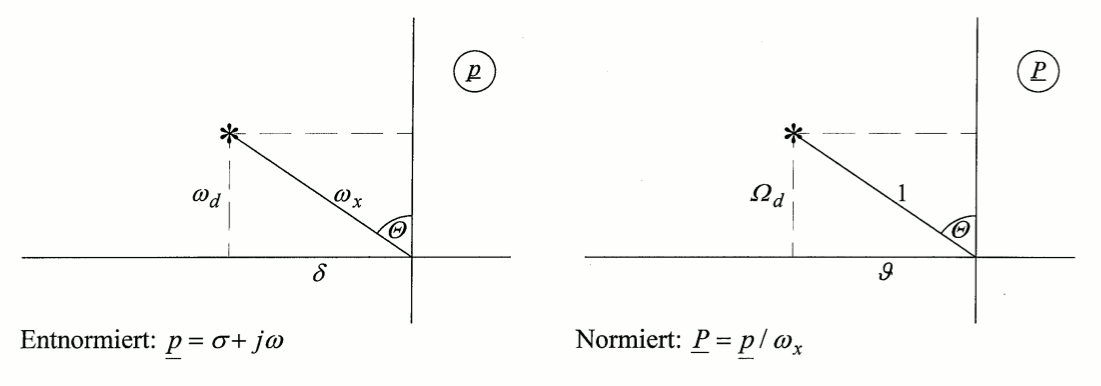
\includegraphics[width=0.9\textwidth]{images/p-ebene.png}
		\caption{Pol in normierter und entnormierter p-Ebene}
	\end{figure}

\clearpage

\section*{Freie, gedämpfte Schwingung}
\subsection*{Definitionen}
    
    \begin{table}[h]
        \begin{tabular}{lll}
        $ Q $ & \multicolumn{2}{l}{\textbf{Güte}} \\
        ~ & $ Q > 0,5 $ & Schwach bedämpft, ausschwingend um Asymtote \\
        ~ & $ Q = 0,5 $ & Maximal flache Näherung an die Asymtote \\
        ~ & $ Q < 0,5 $ & Start bedämpft, von einer Seite der Asymtote annähernd \\
        $ \varTheta $ & \multicolumn{2}{l}{\textbf{Polwinkel}} \\
        $ d $ & \multicolumn{2}{l}{\textbf{Verlustfaktor}} \\
        $ \vartheta $ & \multicolumn{2}{l}{\textbf{Dämpfungsgrad}} \\
        $ \delta $ & \multicolumn{2}{l}{\textbf{Abklingkoeffizient} $ \qquad \delta = Re({\underline{p}}) $} \\
        $ \Lambda $ & \multicolumn{2}{l}{\textbf{Logarithmisches Dekrement}} \\
        ~ & \multicolumn{2}{l}{ist der natürliche Logarithmus der Relation zweier aufeinanderfolgender} \\
        ~ & \multicolumn{2}{l}{Maxima beim Ein- / Ausschwingvorgang. Entspricht Hüllkurve während} \\
        ~ & \multicolumn{2}{l}{einer Periode $ T_d = \nicefrac{1}{f_d} $ in Neper. ($ 1Np = 8,686dB $)} \\
        $ \tau_{HK} $ & \multicolumn{2}{l}{\textbf{Hüllkurvenzeitkonstante}} \\
        $ D $ & \multicolumn{2}{l}{\textbf{Abklingmaß}} \\
        $ B $ & \multicolumn{2}{l}{\textbf{Bandbreite}} \\
        $ \omega_d $ & \multicolumn{2}{l}{\textbf{Ausschwing- / Eigenfrequenz} $ \qquad \omega_d = Im(\underline{p}) $} \\
        \end{tabular}
    \end{table}
    
\subsection*{Umrechnung der Dämpfungparameter}
    
	\begin{table}[h]
    	\def\arraystretch{1.5}
{\large         \begin{tabular}{|c|c|c|c|c|c|c|}
        \hline
        ~ & Q & d & $\vartheta$ & $\delta$ & $\varTheta$ & $\Lambda$ \\ \hline
        $ Q= $ & ~ & $\frac{1}{d}$ & $\frac{1}{2\vartheta}$ & $\frac{\omega_x}{2\delta}$ & $\frac{1}{2 \cdot \sin{\varTheta}}$ & $\frac{\sqrt{4\pi^2+\Lambda^2}}{2\Lambda}$ \\ \hline
        $ d= $ & $\frac{1}{Q}$ & ~ & $2\vartheta$ & $\frac{2\delta}{\omega_x}$ & $2\cdot\sin{\varTheta}$ & $\frac{2\Lambda}{\sqrt{4\pi^2+\Lambda^2}}$ \\ \hline
        $ \vartheta= $ & $\frac{1}{2Q}$ & $\frac{d}{2}$ & ~ & $\frac{\delta}{\omega_x}$ & $\sin{\varTheta}$ & $\frac{\Lambda}{\sqrt{4\pi^2+\Lambda^2}}$ \\ \hline
        $ \delta= $ & $\frac{\omega_x}{2Q}$ & $\frac{\omega_x d}{2}$ & $\vartheta\cdot\omega_x$ & ~ & $\omega_d\cdot\tan{\varTheta}$ & $\Lambda \cdot f_d$ \\ \hline
        $ \varTheta= $ & $\sin^{-1}{\frac{1}{2Q}}$ & $\sin^{-1}{\frac{d}{2}}$ & $\sin^{-1}{\vartheta}$ & $\tan^{-1}{\frac{\delta}{\omega_d}}$ & ~ & $\tan^{-1}{\frac{\Lambda}{2\pi}}$ \\ \hline
        $ \Lambda= $ & $\frac{\pi}{\sqrt{Q^2-\frac{1}{4}}}$ & $\frac{2\pi}{\sqrt{\frac{4}{d^2}-1}}$ & $\frac{2\pi}{\sqrt{\frac{1}{\vartheta^2}-1}}$ & $\frac{\delta}{f_d}$ & $2\pi \cdot \tan{\varTheta}$ & ~ \\ \hline
        \end{tabular}
}    \end{table}

	\begin{minipage}[t]{0.2\textwidth}
		\vspace{-0.2cm}
		\[  \tau_{HK} = \frac{1}{\delta}  \]
	\end{minipage} 
	\begin{minipage}[t]{0.4\textwidth}
		\vspace{-0.4cm}
		\begin{align*}
			D &= \delta \cdot 20dB \cdot \log{e} &\\
			&= \delta \cdot 8,686dB &
		\end{align*}
	\end{minipage}
	\begin{minipage}[t]{0.4\textwidth}
		\vspace{-0.4cm}
		\begin{align*}
			\hat{\omega}_{HP} &= \omega_x \cdot \sqrt{1-2\cdot\vartheta^2} &\\
			\hat{\omega}_{TP} &= \omega_x \cdot \sqrt{1-0.5\cdot\vartheta^2} &
		\end{align*}
	\end{minipage}
	\[ \omega_d = \omega_x \cdot \sqrt{1-\vartheta^2} \]
	
\clearpage

\end{document}
